
% Brief introduction with 
\Gls{pet} is a quantitative imaging technique that makes use of 
positron-emitting radioisotopes for the study of biochemical and physiological processes \textit{in vivo}. The molecules of interest for the studies processes are labelled with a radioisotope and then introduced in the body. The PET imaging system is used to collect information about the location of the labelled molecules \textit{in vivo} and create a map of activity distribution. Information can be collected dynamically over time to track distribution changes with time and deduce information for the characterisation of the underlying process kinetics. 

\subsection{Principles of pharmacokinetic modelling}
Pharmacokinetics refers to the study of absorption, distribution, metabolism and excretion of drugs in living systems. The study of pharmacokinetics is based on measurements of concretion of drugs and their metabolites in tissues over time. Pharmacokinetic models are mathematical relationships, derived from prior knowledge or previous observations, which can be tested against the measurements in order to describe the underlying behaviour. These models describe the transport and binding rates of tracer from local concentration differences across boundaries, that can be either physical (such as a member or an organ outline) or conceptual boundaries as for example for example between bound and unbound tracer. These boundaries define separate compartments with distinct activity concentration which form the basis of the mathematics of pharmacokinetic models, also referred to as compartmental models.\par
\iffalse 
There are three assumptions are made for compartmental modelling to be valid:
The first is the tracer assumption which requires that the presence of the tracer in PET studies is not influencing the physiological processes and molecular interactions. This is the case in most PET studies as the specific activity of the tracer (Activity/tracer concentration) is kept low. The second assumption is that the physiological processes and molecular interactions are in constant state during the duration of the PET study. The third and final assumption is that tracer is homogeneously distributed within each compartment. 
\fi

The three key assumptions underlying compartmental modelling are:
\begin{itemize}
\item  The concentration of the PET tracer is not high enough to influence the physiological processes and molecular interactions under study. 
\item That all physiological processes and interactions are in constant state for the duration of the PET study. 
\item  The assumption that tracer consecration is instantly uniform in all compartments of the model.
\end{itemize}

By common convention in modelling the first compartment is the plasma pool from where the tracer distributes to tissues. The concentration of tracer in the plasma is measured and applied to the model as a known input function that powers the system. If the tracer is metabolised during the study, this needs to be accounted for and the metabolite corrected input function must be used instead. Compartmental models behave according to a set of first-order ordinary differential equations, which means that change of concentration in one compartment is a linear function of the concentrations of all other compartments. This linearity establishes that the measured tissue activity concentration will be the convolution of the input function with the impulse response function (IRF) of the system, which is described by the compartmental model and its parameters. \par
\hl{When a measurement of tissue activity concentration is taken with PET $C_{PET}$, the measurement will include the tissue activity and activity from the intravascular blood in this tissue. The proportion of tissue volume occupied by intravascular blood is $V_B$, which is commonly referred to as simply blood fraction.}\par

\subsection{One-tissue compartment model}
As the simplest model, the two compartment model or one-tissue compartment model (1TCM) can be described using two constant rates for the input and output of tracer from the tissue, $K_1$ and $k_2$ respectively.

\begin{figure}[ht]
	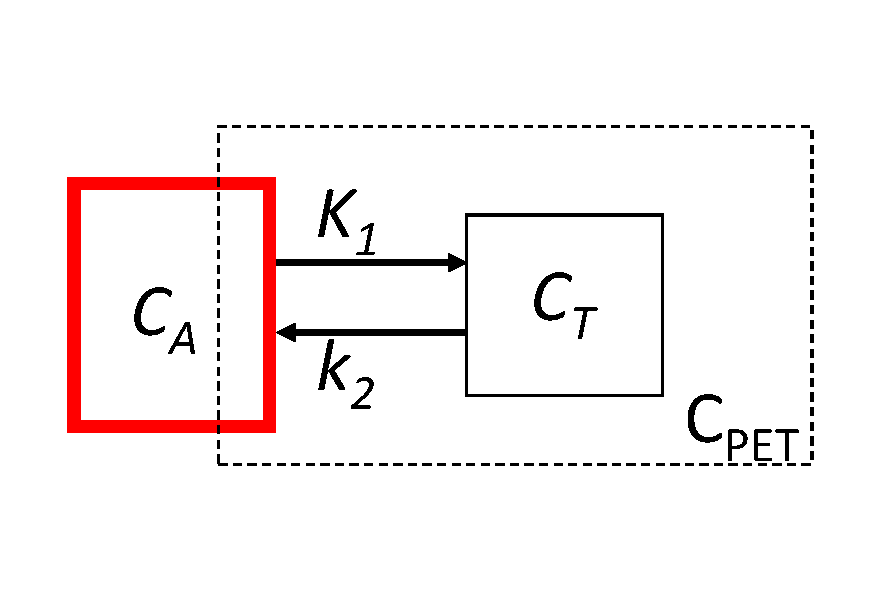
\includegraphics[width=0.4\textwidth]{figures/1_1_1TCM.pdf}
	\centering
	\caption{1 tissue compartment model}
	\centering
	\label{fig:1TCM}
\end{figure}

The rate of change of the activity concentration in tissue $C_T$ will depend on the metabolite corrected arterial input function $C_A$ and the tissue activity concentration in tissue, described by the differential equation \ref{eqn:1TCM_Diff}.

\begin{equation}
  \frac{\mathrm d C_T}{\mathrm d t} = K_1 C_A - k_2 C_T
  \label{eqn:1TCM_Diff}
\end{equation}

\begin{equation}
   C_T = K_1 e^{-k_2 t} \circledast C_A 
  \label{eqn:1TCM}
\end{equation}

\begin{equation}
   C_{PET} =   K_1 e^{-k_2 t} \circledast C_A  (1-V_B) + C_B V_B
  \label{eqn:1TCM_CPET}
\end{equation}

Equation \ref{eqn:1TCM} is the solution of the differential equation \ref{eqn:1TCM_Diff}, which becomes \ref{eqn:1TCM_CPET} for the PET measurement which includes the fractional blood volume. In equation \ref{eqn:1TCM_CPET} it is important to note that the blood fraction is related to the whole blood activity concentration $C_B$ , rather than the metabolite corrected activity concentration $C_A$. When the tracer metabolic activity is negligible and under the assumption of negligible tracer delay and diffusion from arterial to venous blood TACs, the two concentrations ( $C_A = C_B$) can be set equal in favour if simplified models and estimations. 

\subsection{Two-tissue compartment model}
The three compartment model or two-tissue compartment model (2TCM) is a commonly used model as it describes the behaviour of ${}^{18}F$-Fluorodeoxyglucose (${}^{18}\mathrm{F}$-FDG), which is commonly used radiopharmaceutical in clinical PET. The separation into two tissue compartments is made to distinguish between free and trapped tracer, with the trapping caused by the tracer being metabolised by mitochondria to FDG-6-PO4. The reverse pathway of tracer from the trapped to the free state, via the process of dephosphorylation, is commonly neglected as its consider too slow to be significant during the scan duration of PET studies. With the assumption of $k_4=0$ the two differential equations in \ref{eqn:2TCM_Diff} simplify to the system \ref{eqn:2TCM_Diff_k4=0} which when solved results to equation \ref{eqn:2TCM}. 

\begin{subequations}
\begin{align}
C_{PET} = (C_F + C_B)(1-V_B) + V_B C_A \\
\frac{d}{dt}C_F = K_1 C_A - (k_2 + k_3)C_F + k_4 C_B \\ 
\frac{d}{dt}C_B = k_3 C_F - k_4 C_B  
\end{align}
\label{eqn:2TCM_Diff}
\end{subequations}

\begin{subequations}
\begin{align}
\frac{d}{dt}C_F = K_1 C_A - (k_2 + k_3)C_F \\ 
\frac{d}{dt}C_B = k_3 C_F  
\end{align}
\label{eqn:2TCM_Diff_k4=0}
\end{subequations}

\begin{equation}
C_T =  C_F + C_B = K_1 ( e^{-(k_2+k_3)t} + \frac{k_3}{k_2+k_3}(1-e^{-(k_2+k_3)t}))   
\label{eqn:2TCM}
\end{equation}

\begin{equation}
K_i = \frac{K_1 k_3}{k_2+k_3}
\label{eqn:FDG_Ki}
\end{equation}

The parameter $K_i$ is the influx rate constant that for FDG is proportional to the influx rate of glucose. 

\subsection{Graphical Analyses Methods}

\subsubsection{Patlak}
\begin{equation}
{C_{T}}(t) = {K_i} \int_{0}^{t} C_{A}(\tau) d\tau +  {V_{\alpha}} C_{A}(t) \ , \;  t>t_{ss} \ ,
\end{equation}
%
\begin{equation} 
{C_{PET}}(t)  = (1-V_{B}){C_{T}}(t) + V_{B}C_{B}(t),
\end{equation}
%
%
\begin{equation} 
{C_{PET}}(t)  = (1-V_{B}){K_i} \int_{0}^{t} C_{A}(\tau) d\tau +  (1-V_{B}) {V_{\alpha}} C_{A}(t) + V_{B}C_{B}(t).
\end{equation}
Assuming that arterial blood tracer concentration $C_{A}$ is equal to whole blood activity concentration $C_{B}$, the PET measured concentration is modelled as
\begin{equation} 
{C_{PET}}(t)  = (1-V_{B}){K_i} \int_{0}^{t} C_{A}(\tau) d\tau +  ((1-V_{B}) {V_{\alpha}}+ V_{B})C_{A}(t).
\end{equation}
Assuming that the blood fraction $V_B$ is small and $(1-V_B) \xrightarrow[]{}1$, this equation becomes
%
%
\begin{equation} 
{C_{PET}}(t)  = {K_i} \int_{0}^{t} C_{A}(\tau) d\tau +  \underbrace{({V_{\alpha}}+ V_{B})}_{V_D} C_{A}(t).
\end{equation}
%
%
%

\subsection{Linearisation methods}
The analytical solutions of the first order differential equations that describe the compartment models involve exponential terms with all model parameters on the exponents, with the exception of $K_1$. The estimation of the model parameters from measured data requires non-linear fitting methods. These methods, such as the commonly used Marquardt-Levenberg algorithm, are iterative search algorithms which are demanding in execution time, sensitive to variations due to noise and do not guarantee convergence to a global minimum. These factors pose significant limitations on the use of non-linear algorithms, especially in the case of parametric imaging as we will see later on where the search algorithm needs to be applied on every voxel of the series of dynamic images.\par
Assumptions and simplifications can be made by transformation of the models in a form that enables the use of regular linear least-squares fitting, in a process that is named linearisation. Depending on the model and the method used, linearisations can result in forms that allow complete estimation of the model parameters or in forms that provide restricted information about the model. 

\subsubsection{1TCM linearization}
The 1TCM described by the differential equation in \ref{eqn:1TCM_Diff} can be simply transformed by integrating over time which results in the form of equation \ref{eqn:1TCM_Lin}. This can be writen in the form of equation \ref{eqn:1TCM_Lin_2} which cannot be used to describe the model, as $C_T$ appears on both sides of the equation, it can be used to estimate the model parameters $K_1$ and $k_2$ from a simple least-squares linear fit using measured data of $C_T$ and the input function $C_A$. 

\begin{equation}
C_T = K_1 \int_{0}^{t} C_A d\tau  - k_2 \int_{0}^{t} C_T d\tau
\label{eqn:1TCM_Lin}
\end{equation}

\begin{equation}
\frac{C_T}{\int_{0}^{t} C_A d\tau} = K_1 - k_2 \frac{\int_{0}^{t} C_T d\tau}{\int_{0}^{t} C_A d\tau} 
\label{eqn:1TCM_Lin_2}
\end{equation}

If the case of the model applied in perfusion measurements, using an inert and diffusible tracer, the radioactivity of vascular blood inside the measured PET volume can be taken into account by including the arterial volume fraction  $V_A$ of the arterial concentration $C_A$ in the equation. The result solution is the form \ref{eqn:1TCM_Lin_3}, which can be solved using linear least square algorithms.

\begin{equation}
C_{PET} = K_1 \int_{0}^{t} C_A d\tau - k_2 \int_{0}^{t} C_T d\tau + V_A \cdot C_A
\label{eqn:1TCM_Lin_3}
\end{equation}

\subsubsection{2TCM linearization}
The system describing the 2TCM in \ref{eqn:2TCM_Diff} can be integrated twice and following rearrangements be written in the following form, according to the rearrangements from Cai et al. \cite{Cai2002}.   

\begin{equation} \label{microLinearization_with_k4}
C_{PET} = P_1 C_A + P_2 \int_0^t \! C_A \, \mathrm{d}\tau + P_3 \int_0^t \int_0^\tau \! C_A \,\mathrm{d}s \mathrm{d}\tau
+ P_4 \int_0^t \! C_{PET} \, \mathrm{d}\tau + P_5 \int_0^t \int_0^\tau \! C_{PET} \,\mathrm{d}s \mathrm{d}\tau
\end{equation}
\newline From which the kinetic parameters can be extracted as: 
\newline
\begin{equation} \label{ParamsLinearization_with_k4}
K_1=\frac{P_1 P_4 + P_2}{1-P_1} ,\  K_2=- \frac{P_1 P_5 + P_3}{P_1 P_4 + P_2} - P_4 ,\ K_3=-(k_2 + k_4 + P_4) 
,\ K_4=-(P_5/k_2) ,\  V_B = P_1 
\end{equation}

\newline 
if prior knowledge of the kinetics behaviour allows to assume that $k_{4} = 0 $ the relationship becomes: 

\begin{equation} \label{microLinearization_no_k4}
C_{PET} = P_1 C_A + P_2 \int_0^t \! C_A \, \mathrm{d}\tau + P_3 \int_0^t \int_0^\tau \! C_A \,\mathrm{d}s \mathrm{d}\tau
+ P_4 \int_0^t \! C_{PET} 
\end{equation}
\newline From which the kinetic parameters can be extracted as: 
\newline
\begin{equation} \label{ParamsLinearization_no_k4}
K_1=\frac{P_1 P_4 + P_2}{1-P_1} ,\  K_2=- \frac{P_3}{P_1 P_4 + P_2} - P_4 ,\ K_3=\frac{P_3}{P_1 P_4 + P_2} ,\  V_B = P_1
\end{equation}

\subsection{Basis functions method}
For the 2TCM the solution of the system in its general form, with the assumption of $k_4 = 0$, can be re-written according to \cite{Hong2010} as 

\begin{equation} \label{BFM_FullSolution_no_k4}
C_{PET} = (\theta_1 + \theta_2 e^{-\alpha_2 t } ) \otimes C_A + V_B C_B
\end{equation}
\begin{equation} \label{BFM_FullSolution_no_k4_simplified}
C_{PET} = \theta_1 \otimes C_A + \theta_2 e^{-\alpha_2 t } \otimes C_A   + V_B C_B
\end{equation}

In the form of the 2TCM \ref{BFM_FullSolution_no_k4_simplified} the non linear term involving the exponent can estimated via a search within a range of possible values. A large set (for example N=100) basis functions can be pre-calculated for the non-linear term, which can then be used along with a linear least-square solution of the other terms in \ref{BFM_FullSolution_no_k4_simplified_BasisFunctions} to find the solution with the lowest residual sum of squares. From that solution the found $\alpha_2$ parameter and the fitted $\theta_1$ and $\theta_2$ can be used to estimate the 2TCM microparameters using

\begin{equation} \label{BFM_FullSolution_no_k4_simplified_BasisFunctions}
C_{PET} = \theta_1 \int_0^t \! C_A \, \mathrm{d}\tau + \theta_2 B_{2j}   + V_B C_B
\end{equation}

\begin{equation} \label{BasisFunctions}
B_{2j} = e^{-\alpha_2 t } \otimes C_A   \ \ ; \  j=1..N \textrm{ for different } \alpha_2 \in [0.06,0.6]min^{-1}
\end{equation}


\begin{subequations}
\begin{align}
K_1 = \frac{\theta_1 + \theta_2}{1-V_b} \\
k_2 = \frac{\theta_2\alpha_2}{\theta_1 + \theta_2} \\
k_3 = \frac{\theta_1\alpha_2}{\theta_1 + \theta_2}
\end{align}
\label{eqn:FDG_microparameters}
\end{subequations}

\subsection{Spectral analysis method - Basis pursuit}
The Spectral analysis method was originally introduced by Cunningham et al. \cite{Cunningham1993}. The method is based on the general from of solutions of compartmental modelling which is a sum of spectral functions. Using this general form the model an be estimated by convolution of the exponential functions with the input function. The fitted spectral model can be used to deduce information about the underlying kinetics, the number of compartments and model macroparameters.

\hl{Previous text to use/edit}

The behaviour of the imaging system is: 

\begin{equation} \label{EqRE}
C_{PET} = (1-V_B) C_T + V_B C_B
\end{equation}


where the $C_T$ can now be modelled with exponentials 

\begin{equation} \label{EqRE}
C_{T} = IRF(t) \otimes C_A 
\end{equation}

\begin{equation} \label{IRF}
IRF(t) = \sum_{j=0}^{M} \phi_j e^{-\beta_j t}\
\end{equation}

\newline The estimated spectral components assume different meaning depending on the position of the $\beta$ grid where they are located. When $\beta_j$ is very high ( $\lim_{j\to\infty} \beta_j$ ) the exponential is approximated by a delta function and represents free passage of tracer. When $\beta_j$ is very low ( $\beta_j=0$ ) the exponential is equal to 1 and represents full trapping of the tracer. 

\newline We will use $\beta_{M+1} = \lim_{j\to\infty} \beta_j$ and $\beta_0 = 0 $. 
The tissue response function becomes:

\begin{equation} \label{EqRE}
IRF(t) = \phi_0 + \sum_{j=1}^{M} \phi_j e^{-\beta_j t} 
\end{equation}

and thus $C_T$ can be expressed as 

\begin{equation} \label{EqRE}
C_{T}  = \phi_0  \int_{0}^{t}C_A  d\tau + \sum_{j=1}^{M} \phi_j e^{-\beta_j t} \otimes C_A 
\end{equation}

, where $\int_{0}^{t}C_A  d\tau$ represents full trapping of tracer.

For the PET measurement we have: 

\begin{equation} \label{EqRE}
C_{PET} = ( \phi_0  \int_{0}^{t}C_A  d\tau + \sum_{j=1}^{M} \phi_j e^{-\beta_j t} \otimes C_A  )(1-V_B) + V_B C_B
\end{equation}

\newline
if we assume  $(1-V_B)\approx1$ then:

\begin{equation} \label{EqRE}
C_{PET} = \phi_0\int_{0}^{t}C_Ad\tau  + \sum_{j=1}^{M} \phi_j e^{-\beta_j t} \otimes C_A  + V_B C_B
\end{equation}

Now assuming that the tracer is not metabolised and $C_A = C_B$, and re-write $V_B$ as $\phi_{M+1}$

\begin{equation} \label{EqRE}
C_{PET} = \phi_0\int_{0}^{t}C_Ad\tau  + \sum_{j=1}^{M} \phi_j e^{-\beta_j t} \otimes C_A  + \phi_{M+1} C_A
\end{equation}

\newline where $\phi_0$ represents trapping of the tracer, $\phi_j$ the M spectral coefficients that describe the equilibrating components (equal to the number of compartments in the system) and $\phi_{M+1}$ the blood fraction

For representation purposes this equation can be re-written in a generic form 

\begin{equation} \label{EqRE}
C_{PET} = \sum_{j=0}^{M+1} \phi_j e^{-\beta_j t} \otimes C_A 
\end{equation}
